The transport of a scalar according to a parabolic function and 
submitted to a monophase flow of a Newtonian and incompressible fluid 
with a high number of \textit{Reynolds} 
($\textit{Re} \rightarrow \infty$) is known as a 
\textit{Pure Advection flow}. In this type of flow, 
it is expected that the scalar will not diffuse. 
For approximation methods like \textit{FEM} and \textit{FDM}, 
it is possible to observe the presence of spurious oscillations. 
As mentioned earlier, several schemes can be used to reduce these 
numerical oscillations. In this section, we will present the use 
of the \textit{semi-Lagrangian} method to reduce spurious oscillations.
In addition, it will be compared to the analytical solution for an
unstructured linear and quadratic triangular mesh 
in order to analyze the numerical diffusion due to the interpolation
as mentioned in the section \ref{discretizacao tempo}. 
The \ref{conveccao} presents schematically the problem and 
the dynamics of scalar transport.

\vspace{0.5cm}
\begin{figure}[H]
\caption{Transport of a scalar in Pure Advection Flow.}
\begin{center}
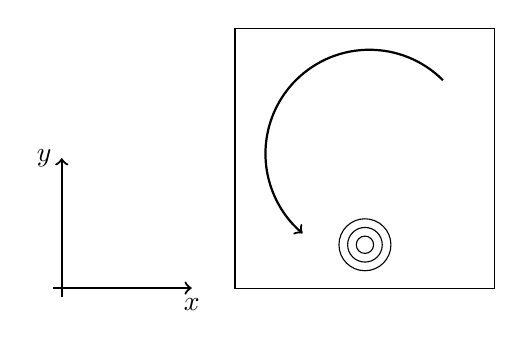
\begin{tikzpicture}[scale=1.1]
 \draw (0,0) -- (3,0) -- (3,3) -- (0,3) -- cycle;

 \draw [->,thick] (2.4,2.4) arc (45:230:1.2);
 
 \draw [->,thick] (-2,-0.1)--(-2,1.5) node[left] {$y$};
 \draw [->,thick] (-2.1,0)--(-0.5,0) node[below] {$x$};

 \draw (1.5,0.5) circle (0.3);
 \draw (1.5,0.5) circle (0.2);
 \draw (1.5,0.5) circle (0.1);

\end{tikzpicture}
\end{center}
\label{conveccao}
\end{figure}

\medskip
\noindent
The scalar transport $\alpha$ for a pure advection flow is shown below:


\begin{equation}
 \frac{\partial \alpha}{\partial t} 
 + 
 \textbf{v} \cdot \nabla \alpha
 = 0
\end{equation}

\noindent
where $\textbf{v} = (u,v)$ is velocity field and its components are
defined as: $u = -y$ e $v = x$. 
Therefore, it is expected that given an initial scalar field, 
it will be displaced by the velocity field without diffusion, 
that is, its profile should not be changed while the flow occurs. 
Any change in the scalar field profile is considered a numerical error.
For this numerical simulation, the domain was discretized using an
unstructured linear triangular mesh with 2216 nodes and 4270 elements
and an unstructured quadratic triangular mesh with 8701 nodes 
and 4270 elements.
In addition to the initial scalar field was defined by a parabolic
profile $c = 1 - x^2 - y^2$, where $x$ and $y$ are space components.



\medskip
The \ref{SL linear} shows the comparison between the scalar field
profile $\alpha$ for the numerical solution using the semi-Lagrangian 
Method in an unstructured linear triangular mesh 
and the analytical solution in 
several positions on the axis of rotation as the flow occurs. 
As can be seen, the spurious oscillations are not observed,
however the scalar field profile in semi-Lagrangian Method
is diffused due to the interpolation. Therefore, for this problem,
the semi-Lagrangian Method in an unstructured linear triangular mesh
did not present a satisfactory result.


\begin{center}
\begin{figure}[H]
     \caption{Comparison of $\alpha$ profile for the semi-Lagrangian Method and analytical solution in several positions on the axis of rotation using an unstructured linear triangular mesh} 
     \centering
     \begin{minipage}{.5\linewidth}
      \centering
      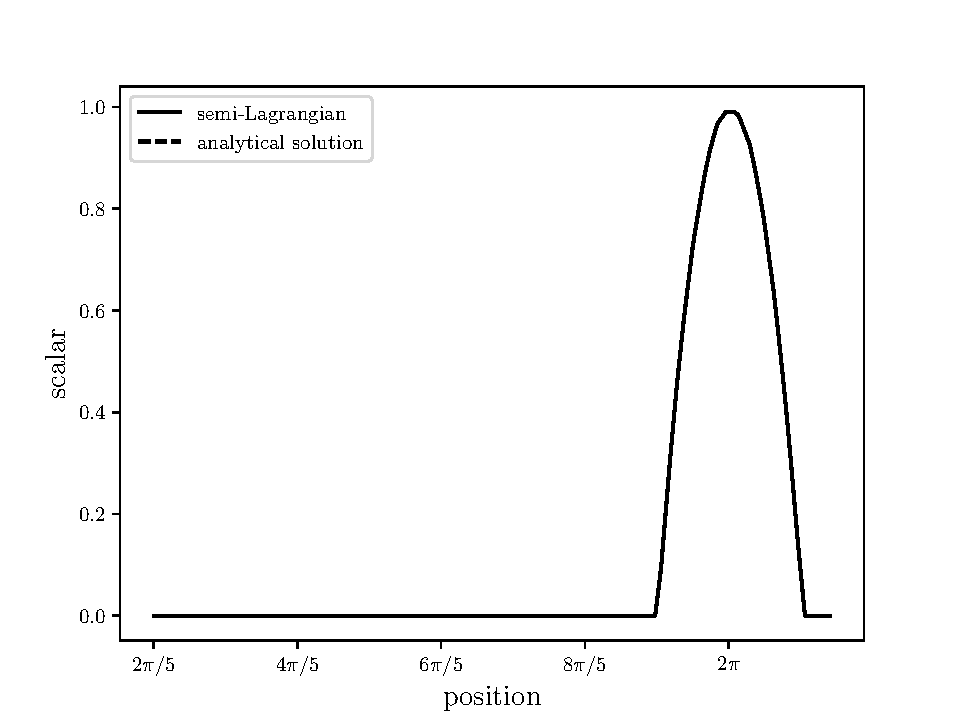
\includegraphics[scale=0.53]{./02_chaps/cap_validation/figure/SLlinear0.pdf}\\
      (a) initial
     \end{minipage}%
     \begin{minipage}{.5\linewidth}
      \centering
      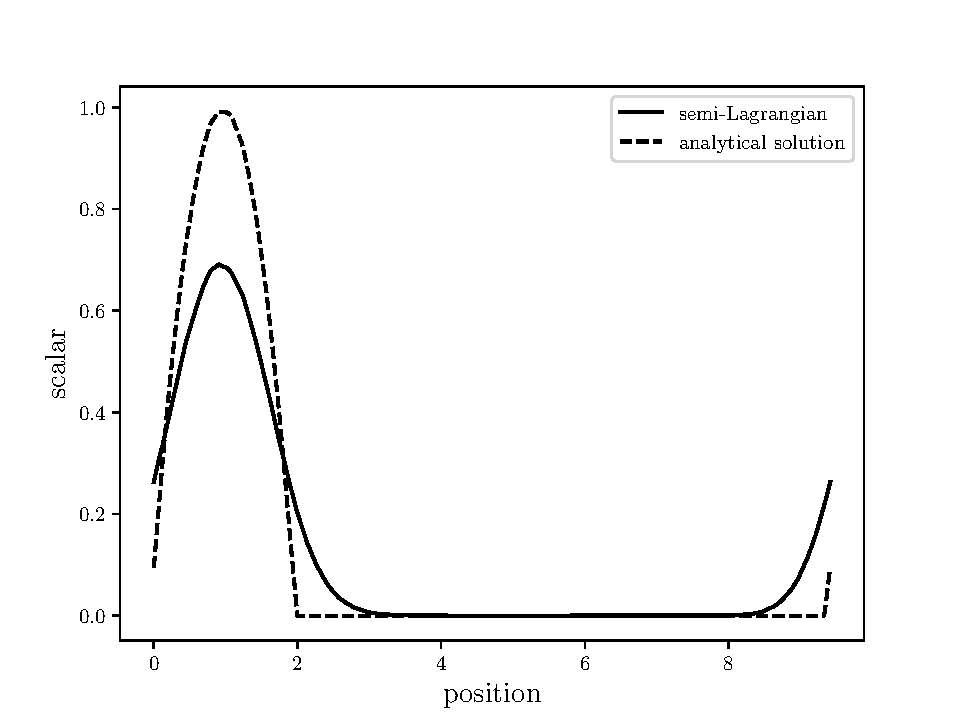
\includegraphics[scale=0.53]{./02_chaps/cap_validation/figure/SLlinear1.pdf}\\
      (b) 1/4 rotation
     \end{minipage}
     \begin{minipage}{.5\linewidth}
      \centering
      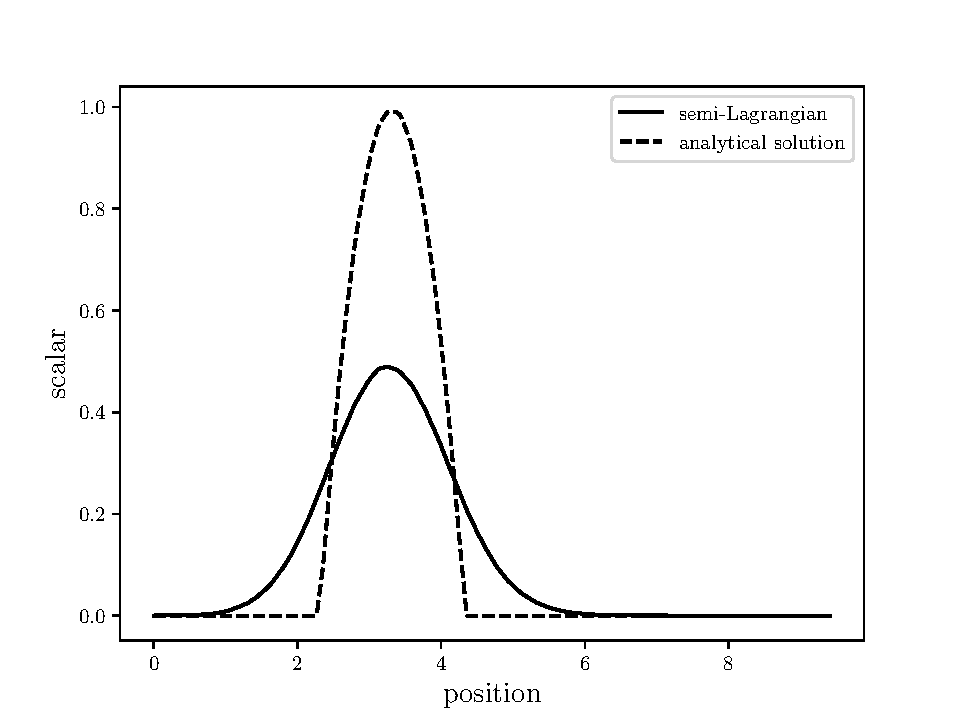
\includegraphics[scale=0.53]{./02_chaps/cap_validation/figure/SLlinear2.pdf}\\
      (c) 1/2 rotation
     \end{minipage}%
     \begin{minipage}{.5\linewidth}
      \centering
      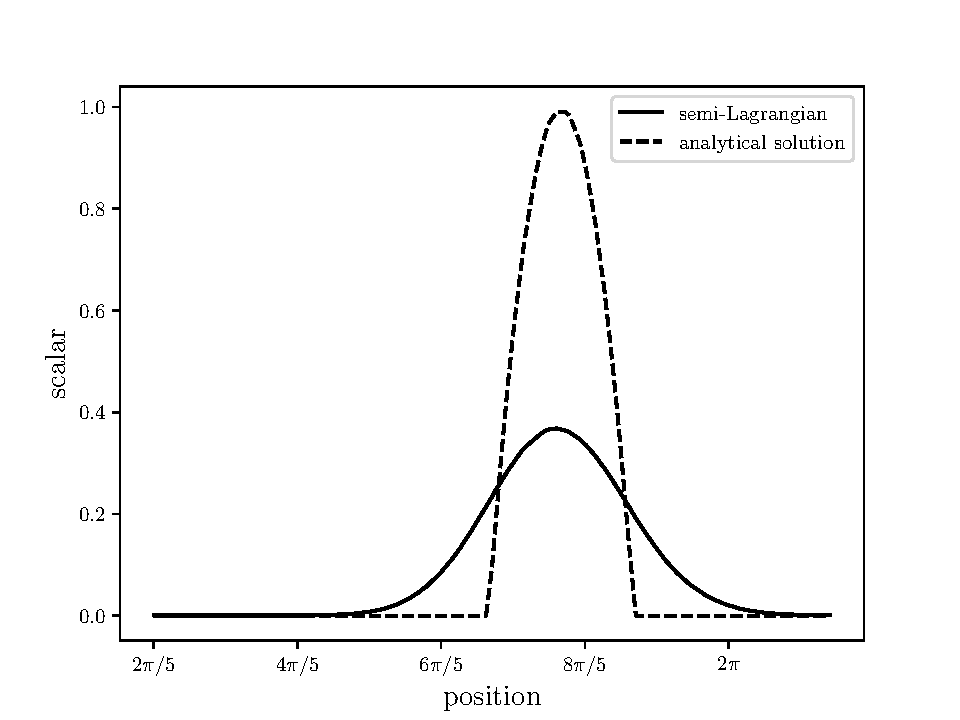
\includegraphics[scale=0.53]{./02_chaps/cap_validation/figure/SLlinear3.pdf}\\
      (d) 3/4 rotation
     \end{minipage}
     \label{SL linear}
\end{figure}
\end{center}


\medskip
The \ref{SL quad} shows the 
comparison between the semi-Lagrangian and analytical solution
for the same previously scalar field
profile $\alpha$,
however an unstructured quadratic triangular mesh is used.
As can be seen, the scalar field profile in semi-Lagrangian Method
shows low numerical diffusion and 
the numerical result is better than the previous one.
In addition, the spurious oscillations are not observed.
Therefore, for this problem,
the semi-Lagrangian Method in an unstructured quadratic triangular mesh
present a satisfactory result.


\begin{center}
\begin{figure}[H]
     \caption{Comparison of $\alpha$ profile for the semi-Lagrangian Method and analytical solution in several positions on the axis of rotation using an unstrutured quadratic triangular mesh} 
     \centering
     \begin{minipage}{.5\linewidth}
      \centering
      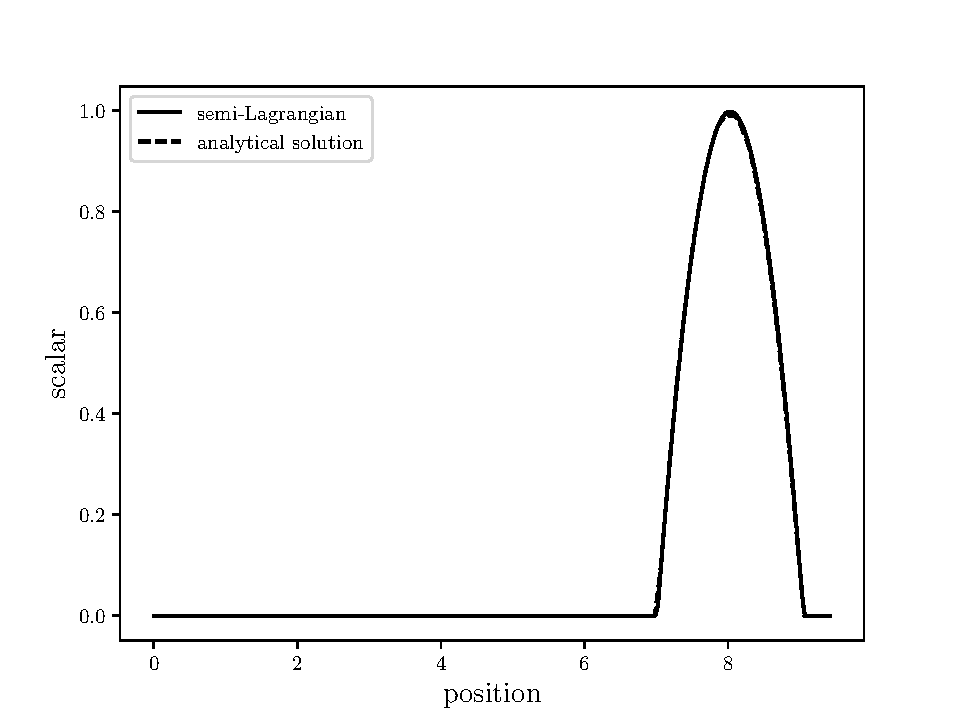
\includegraphics[scale=0.53]{./02_chaps/cap_validation/figure/SLquad0.pdf}\\
      (a) initial
     \end{minipage}%
     \begin{minipage}{.5\linewidth}
      \centering
      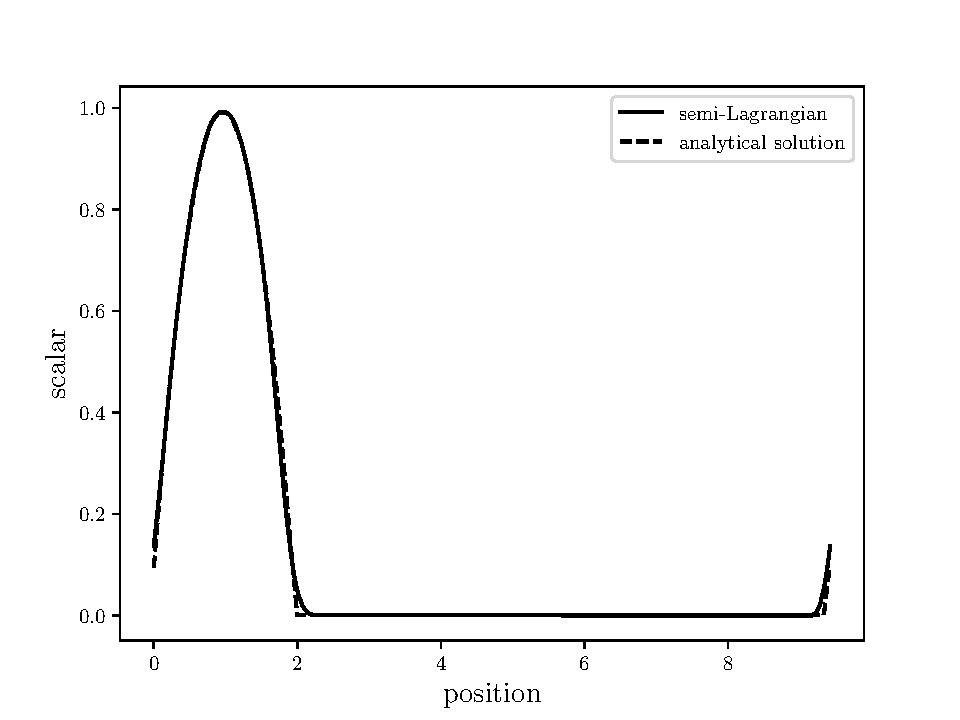
\includegraphics[scale=0.53]{./02_chaps/cap_validation/figure/SLquad1.pdf}\\
      (b) 1/4 rotation
     \end{minipage}
     \begin{minipage}{.5\linewidth}
      \centering
      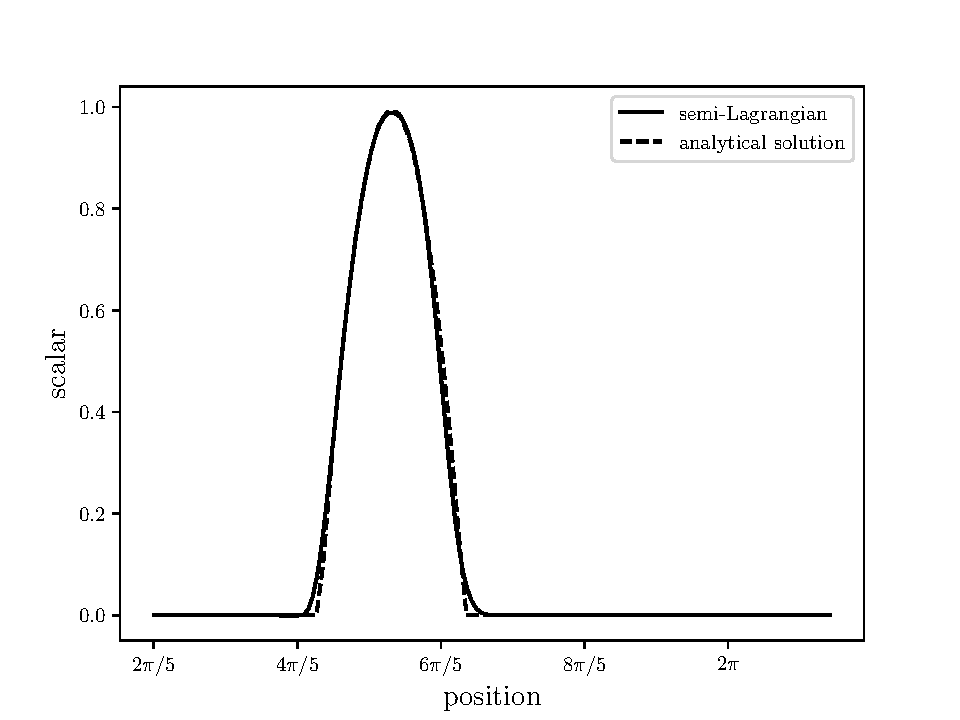
\includegraphics[scale=0.53]{./02_chaps/cap_validation/figure/SLquad2.pdf}\\
      (c) 1/2 rotation
     \end{minipage}%
     \begin{minipage}{.5\linewidth}
      \centering
      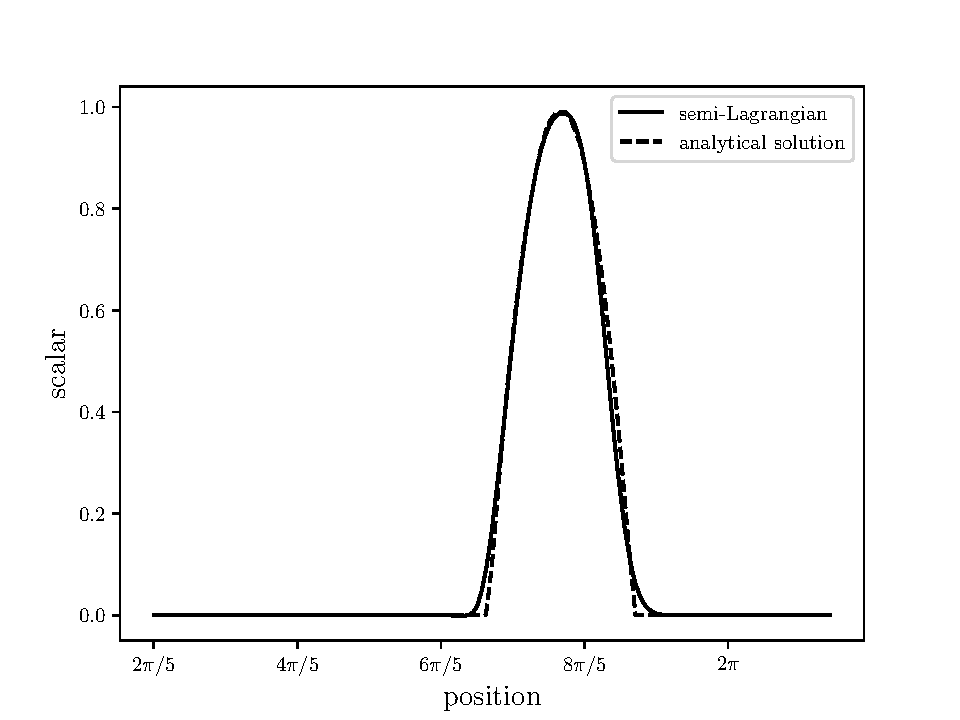
\includegraphics[scale=0.53]{./02_chaps/cap_validation/figure/SLquad3.pdf}\\
      (d) 3/4 rotation
     \end{minipage}
     \label{SL quad}
\end{figure}
\end{center}






\vspace{-1cm}
The \ref{SL linear fig} and \ref{SL quad fig} 
show the spatial and temporal evolution
of the scalar profile for the semi-Lagrangian Method in an
unstructured linear and quadratic triangular mesh  
respectively. As mentioned earlier, the spurious oscillations 
are not presented in both simulations. 
However, in the \ref{SL linear fig}, it is possible
to observe the numerical diffusion, making its use not
recommended for high Reynolds number problem.

\vspace{0.5cm}
\begin{figure}[H]
     \caption{
Spatial and temporal evolution for the semi-Lagrangian Method in several positions of the axis of rotation using an unstructured linear triangular mesh}	
     \centering
     \begin{minipage}{.5\linewidth}
      \centering
      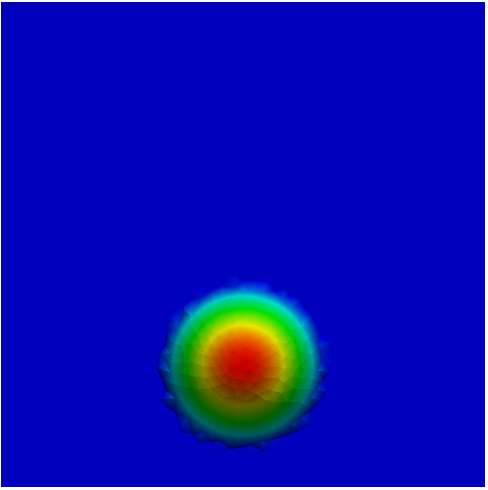
\includegraphics[scale=0.42]{./02_chaps/cap_validation/figure/figSLlinear0.png}\\
      (a) inital
     \end{minipage}%
     \begin{minipage}{.5\linewidth}
      \centering
      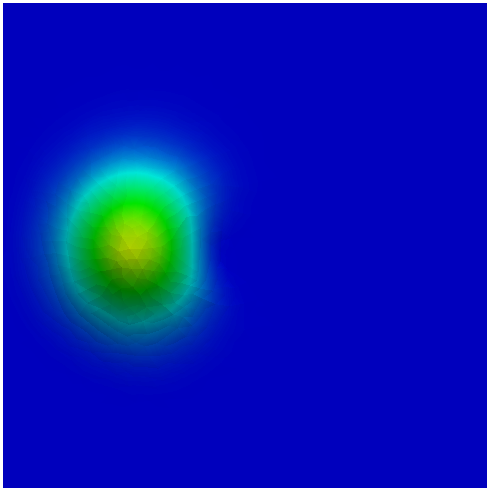
\includegraphics[scale=0.42]{./02_chaps/cap_validation/figure/figSLlinear1.png}\\
      (b) 1/4 rotation
     \end{minipage}\\[10pt]
     \begin{minipage}{.5\linewidth}
      \centering
      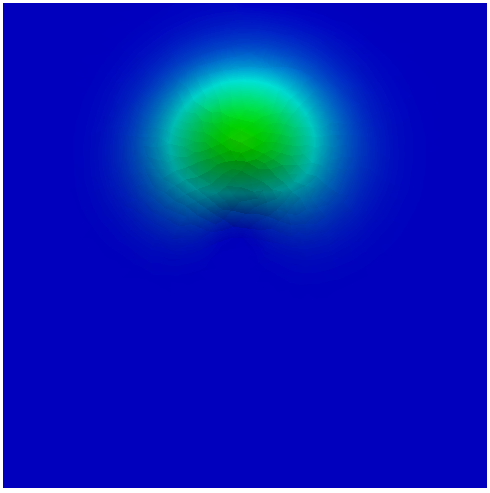
\includegraphics[scale=0.42]{./02_chaps/cap_validation/figure/figSLlinear2.png}\\
      (c) 1/2 rotation
     \end{minipage}%
     \begin{minipage}{.5\linewidth}
      \centering
      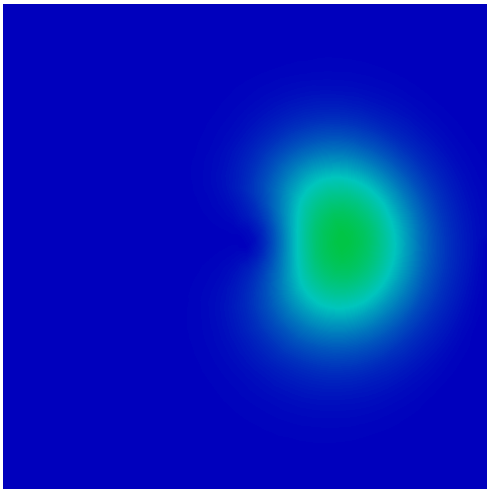
\includegraphics[scale=0.42]{./02_chaps/cap_validation/figure/figSLlinear3.png}\\
      (d) 3/4 rotation
     \end{minipage}
     \label{SL linear fig}
\end{figure}


\vspace{0.5cm}
\begin{figure}[H]
     \caption{
Spatial and temporal evolution for the semi-Lagrangian Method in several positions of the axis of rotation using an unstructured quadratic triangular mesh}	
     \centering
     \begin{minipage}{.5\linewidth}
      \centering
      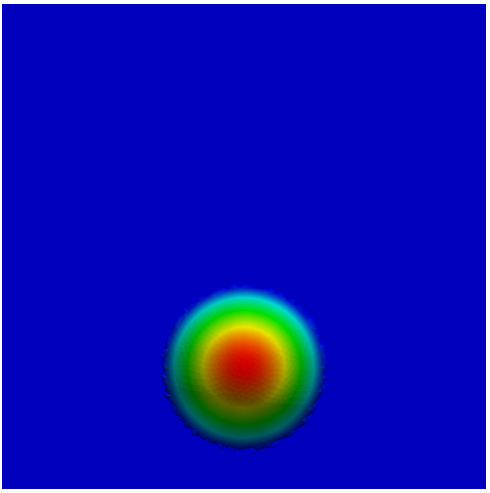
\includegraphics[scale=0.42]{./02_chaps/cap_validation/figure/figSLquad0.png}\\
      (a) initial
     \end{minipage}%
     \begin{minipage}{.5\linewidth}
      \centering
      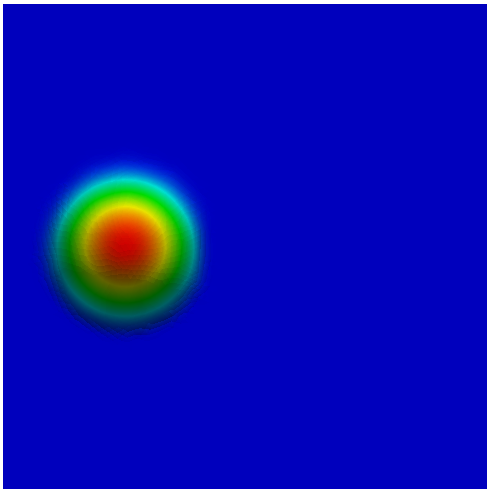
\includegraphics[scale=0.42]{./02_chaps/cap_validation/figure/figSLquad1.png}\\
      (b) 1/4 rotation
     \end{minipage}\\[10pt]
     \begin{minipage}{.5\linewidth}
      \centering
      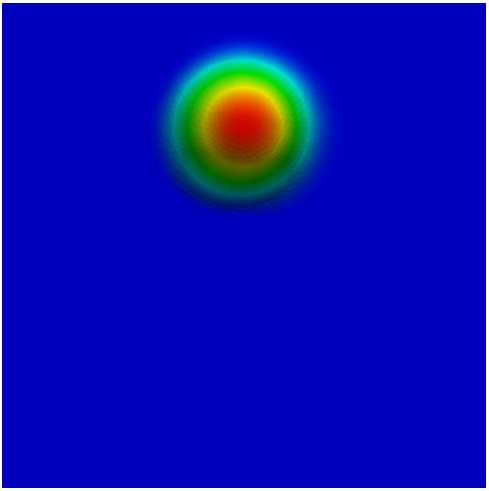
\includegraphics[scale=0.42]{./02_chaps/cap_validation/figure/figSLquad2.png}\\
      (c) 1/2 rotation
     \end{minipage}%
     \begin{minipage}{.5\linewidth}
      \centering
      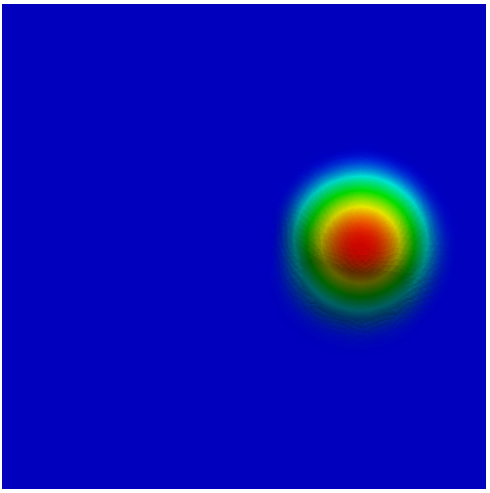
\includegraphics[scale=0.42]{./02_chaps/cap_validation/figure/figSLquad3.png}\\
      (d) 3/4 rotation
     \end{minipage}
     \label{SL quad fig}
\end{figure}

